\documentclass{beamer}

\usepackage[utf8]{inputenc}
\usepackage{algorithm2e, amsmath}
\usepackage{color}
\usepackage{comment}
\usepackage{tikzit}
\usepackage{amsthm}
\usepackage{hyperref}
\input{pq1.tikzstyles}

\usetheme{Rochester}
\usefonttheme{serif}
\usecolortheme{rose}

\title{Spanning Tree Problem With Constraint on the Number of Leaves}
\author{17050\{02,17,66,92,94\} \\ Department of CSE, BUET}

\date{January 8, 2023}

\AtBeginSection[]
{
  \begin{frame}<beamer>
    \frametitle{Outline}
    \tableofcontents[currentsection]
  \end{frame}
}
\AtBeginSubsection[]
{
  \begin{frame}<beamer>
    \frametitle{Outline}
    \tableofcontents[currentsection, currentsubsection]
  \end{frame}
}

% https://cs.stackexchange.com/questions/108801/is-maximum-leaves-spanning-tree-np-complete 

% https://github.com/farvaresh/Benchmarks-for-Maximum-Leaf-Spanning-Tree-Problem-with-an-Application-in-the-Forest-Fire-Detection 



\begin{document}

\begin{frame}
\centering
\maketitle
\end{frame}

\section{Definitions}


\begin{frame}{Spanning Tree}
\begin{figure}
  \tikzfig{w7_1}
  \vspace{1 cm}
  \caption{The Graph $W_7$}
\end{figure}
\end{frame}
\begin{frame}{Spanning Tree}
\begin{figure}
  \tikzfig{w7_2}
  \vspace{1 cm}
  \caption{A Spanning Tree of $W_7$ with $2$ leaves}
\end{figure}
\end{frame}
\begin{frame}{Spanning Tree}
\begin{figure}
  \tikzfig{w7_3}
  \vspace{1 cm}
  \caption{A Spanning Tree of $W_7$ with $6$ leaves}
\end{figure}
\end{frame}

\begin{frame}{Problems: Optimization Versions}

\begin{exampleblock}{Minimum Leaf Spanning Tree Problem}
 Given a connected graph $G$, find a spanning tree of $G$ with the \textbf{minimum} number of leaves.
\end{exampleblock}
\vspace{0.7 cm}
\begin{exampleblock}{Maximum Leaf Spanning Tree Problem}
 Given a connected graph $G$, find a spanning tree of $G$ with the \textbf{maximum} number of leaves.
\end{exampleblock}

\end{frame}

\begin{frame}{Problems: Decision Versions}

\begin{exampleblock}{Minimum Leaf Spanning Tree Problem \textsc{(MinLST)}}
 Given a connected graph $G$ and an integer $k$, does $G$ have a spanning tree with \textbf{at most} $k$ leaves?
\end{exampleblock}
\vspace{0.7 cm}
\begin{exampleblock}{Maximum Leaf Spanning Tree Problem \textsc{(MaxLST)}}
 Given a connected graph $G$ and an integer $k$, does $G$ have a spanning tree with \textbf{at least} $k$ leaves?
\end{exampleblock}

\end{frame}
\begin{comment}
\begin{frame}{Problems: Decision Versions}
    \begin{block}{Both problems are in $\mathcal{NP}$}
    For either problem, given a YES-certificate, we can verify in polynomial time.
    \end{block}
\end{frame}

\end{comment}


\section{Intractability of the Problems}

\begin{frame}{Section Overview}
    \begin{block}{\textsc{MinLST} and \textsc{MaxLST}: Both problems are in $\mathcal{NP}$}
    For either problem, given a YES-certificate, we can verify in polynomial time.
    \end{block} 

    \vspace{0.5 cm}
    Now we will reduce known $\mathcal{NP}$-hard problems to our problems to show them to be $\mathcal{NP}$-hard. 
    \begin{enumerate}
        \item {\textsc{HamPath} $\leq_{P}$ \textsc{MinLST}} 
        \item {\textsc{VertexCover} $\leq_{P}$ \textsc{MinConDomSet} $\leq_{P}$ \textsc{MaxLST}}
    \end{enumerate}
\end{frame}

\subsection{Minimum Leaf Spanning Tree}

\begin{comment}
\begin{frame}{\textsc{MinLST}}

\begin{lemma}
  \textsc{HamPath} $\leq_{P}$ \textsc{MinLST}
\end{lemma}
\pause
\vspace{0.4 cm}
Question 1: Given a connected graph $G$, does $G$ have a Hamiltonian path? \\ \vspace{0.4 cm}
Question 2: Given a connected graph $G$, does $G$ have a spanning tree of at most $2$ leaves?
\end{frame}
\end{comment}


\begin{frame}{\textsc{HamPath} $\leq_{P}$ \textsc{MinLST}}
\begin{figure}
  \tikzfig{w7_2}
  \vspace{0.3 cm}

  \caption{\small A Spanning Tree of $W_7$ with at most $2$ leaves which is also a Hamiltonian Path}
\end{figure} \pause 
\begin{lemma}
    A connected graph $G$ has a Hamiltonian path if and only if it has a spanning tree of at most two leaves. 
\end{lemma}
\end{frame}

\subsection{Maximum Leaf Spanning Tree}


\begin{frame}{Connected Dominating Set}

\begin{figure}
\scalebox{0.7}{
  \tikzfig{w7_4}
}
  \caption{The red vertices form a Connected Dominating Set}
\end{figure}
\pause
\begin{definition}
 Given a graph $G=(V, E)$, a connected dominating set $S \subseteq V$ is such that
 \begin{enumerate}
  \item For every vertex $u \in V$, either $u \in S$ or $u$ has a neighbor $v \in S$.
  \item The subgraph of $G$ induced by $S$ is connected.
 \end{enumerate}
\end{definition}


\end{frame}

\begin{frame}{\textsc{MinCDS}}
   \begin{exampleblock}{Minimum Connected Dominating Set: Decision Version}
     Given a connected graph $G$ and an integer $k$, does $G$ have a connected dominating set of size \textbf{at most} $k$?
   \end{exampleblock} 

   \begin{block}{\textsc{MinCDS} $\leq_{P}$ \textsc{MaxLST}} 
   A connected graph $G$ has a connected dominating set of size at most $k$ if and only if it has a spanning tree of at least $n-k$ leaves. 
   \end{block}
   % \begin{comment}
   % explain something along the way of:
   %     Given a sequence of vertices forming a Connected Dominating Set in the graph. We can validate this solution by checking that all the vertices belong to the vertices of the graph and all the vertices that are not a part of this sequence are adjacent to some of the vertex in this set. This can be done in polynomial time, that is O(V +E) using the following strategy
   %      flag=true
   %      for every vertex v in V:
   %        if v doesn't belong to Dominating Set:
   %           verify the set of edges 
   %           corresponding to v 
   %           if v is not adjacent 
   %              to any of the vertices in DS, 
   %              set flag=False and break
   %      if (flag)
   %         solution is correct
   %      else
   %         solution is incorrect
   % \end{comment}
\end{frame}



\begin{frame}{Minimum Connected Dominating Set}
\only<1>{
    \begin{figure}
    \scalebox{1.5}{
      \tikzfig{graph-G}
    }
      \caption{The maximum leaf spanning tree(MaxLST) is equivalent to the minimum connected dominating set(MinCDS)}
    \end{figure}
    }
\only<2>{
    \begin{figure}
    \scalebox{1.5}{
      \tikzfig{graph-G-mincds}
    }
      \caption{The maximum leaf spanning tree(MaxLST) is equivalent to the minimum connected dominating set(MinCDS)}
    \end{figure}
    }
\only<3>{
    \begin{figure}
    \scalebox{1.5}{
      \tikzfig{graph-G-maxlst}
    }
      \caption{The maximum leaf spanning tree(MaxLST) is equivalent to the minimum connected dominating set(MinCDS)}
    \end{figure}
    }
\end{frame}

\begin{frame}{\textsc{MinCDS}}
   \begin{exampleblock}{Minimum Connected Dominating Set: Decision Version}
     Given a connected graph $G$ and an integer $k$, does $G$ have a connected dominating set of size \textbf{at most} $k$?
   \end{exampleblock} 

   \begin{block}{\textsc{MinCDS} $\leq_{P}$ \textsc{MaxLST}} 
   A connected graph $G$ has a connected dominating set of size at most $k$ if and only if it has a spanning tree of at least $n-k$ leaves. 
   \end{block}
   % \begin{comment}
   % explain something along the way of:
   %     Given a sequence of vertices forming a Connected Dominating Set in the graph. We can validate this solution by checking that all the vertices belong to the vertices of the graph and all the vertices that are not a part of this sequence are adjacent to some of the vertex in this set. This can be done in polynomial time, that is O(V +E) using the following strategy
   %      flag=true
   %      for every vertex v in V:
   %        if v doesn't belong to Dominating Set:
   %           verify the set of edges 
   %           corresponding to v 
   %           if v is not adjacent 
   %              to any of the vertices in DS, 
   %              set flag=False and break
   %      if (flag)
   %         solution is correct
   %      else
   %         solution is incorrect
   % \end{comment}
\end{frame}

\begin{frame}{\textsc{VertexCover} $\leq_{P}$ \textsc{MinCDS}}
    \begin{figure}
    \scalebox{1.3}{
        \tikzfig{graph-G}
    }
      \caption{An instance of \textsc{VertexCover}}
    \end{figure}
    \begin{itemize}
        \item An instance $(G(V,E),k)$ of \textsc{VertexCover}
    \end{itemize} concepts
\end{frame}

\begin{frame}{\textsc{VertexCover} $\leq_{P}$ \textsc{MinCDS}}
    \begin{figure}
    \scalebox{1.3}{
      \tikzfig{graph-G-prime}
    }
      \caption{Constructed instance of \textsc{MinCDS}}
    \end{figure}
    \only<1>{
        \begin{itemize}
            \item Constructed instance $(G'(V',E'),k)$ of \textsc{MinCDS}
        \end{itemize}
    }
    \only<2>{
        \begin{itemize}
            \item $V' = V \cup \{x_{uv} : (u,v) \in E\}$
            \item $E' = E \cup \{ (u, v) : u, v \in V, u \neq v, (u,v) \notin E \} \cup \{(x_{u,v},u) : (u,v) \in E\}$
        \end{itemize}
    }
    % \only<3>{
    %     \begin{itemize}
    %         \item Note that any induced subgraph in $G$ is a connected graph in $G'$.
    %     \end{itemize}
    % }

\end{frame}

\begin{frame}{\textsc{VertexCover} $\leq_{P}$ \textsc{MinCDS}}
    \begin{lemma}
        $G$ has a vertex cover of size at most $k$ if and only if $G'$ has a connected dominating set of size at most $k$.
    \end{lemma}
\end{frame}

\begin{frame}{Necessity}
\begin{figure}
    \scalebox{1.3}{
      \tikzfig{graph-G-prime-S}
    }
      \caption{\textsc{VertexCover} of $G$}
    \end{figure}
    \begin{itemize}
        \item $S$ is a \textsc{VertexCover} of $G$
    \end{itemize}
\end{frame}

\begin{frame}{Necessity}
\begin{columns}
    \begin{column}{0.5\textwidth}
        \begin{itemize}[<+->]
            \item for any $v \in V' \setminus S$
            \item Case 1: $v\in V$
            %  by the definition of vertex cover we know that $v$ dominated by $S$
            \item Case 2: $v = v_{xy}$, an edge vertex of some edge $(x,y)\in E$
            % because $(x,y)$ is covered by $S$, then $x\in S$ or $y\in S$, $v_{xy}$ is dominated by $S$. Thus $S$ is a connected dominating set of $G'$.S
        \end{itemize}
    \end{column}
    \begin{column}{0.5\textwidth}
        \begin{figure}
            \scalebox{1.3}{
              \tikzfig{graph-G-prime-S}
            }
            \caption{\textsc{VertexCover} of $G$}
        \end{figure}
    \end{column}
\end{columns}
\end{frame}

\begin{frame}{Sufficiency}
\begin{figure}
    \scalebox{1.3}{
      \tikzfig{graph-G-prime-S-xy}
    }
      \caption{\textsc{CDS} of $G'$}
    \end{figure}
    \begin{itemize}
        \item $S$ is a \textsc{CDS} of $G'$
    \end{itemize}
\end{frame}

\begin{frame}{Sufficiency}
\begin{figure}
    \scalebox{1.3}{
      \tikzfig{graph-G-prime-S}
    }
      \caption{\textsc{CDS} of $G'$}
\end{figure}
    \begin{itemize}
        \item For any edge vertex $v_{xy}\in S$, we replace it with $x$ or $y$.
    \end{itemize}
\end{frame}

\begin{frame}{Sufficiency}
\begin{figure}
    \scalebox{1.3}{
      \tikzfig{graph-G-prime-S}
    }
      \caption{\textsc{CDS} of $G'$}
\end{figure}
    \begin{itemize}[<+->]
        \item $S$ contains no edge vertex
        \item every edge vertex is dominated by $S$
        \item $S$ is a vertex cover for $G$
    \end{itemize}
\end{frame}



\section{Algorithms to Explore}

\begin{frame}{\textsc{MaxLST}}
    \begin{enumerate}
        \item<1->An $\mathcal{O}^*(1.8966^n)$ exact algorithm by  Fernau et al. (2009)
        \item<2->A $2$-approximation algorithm by Solis-Oba et al. (2017) 
        \item<3->\textsc{MaxLST} is APX-hard, and thus no PTAS exists unless $\mathcal{P}=\mathcal{NP}$. (Galbiati et al., 1994)
        \item<4->An $\mathcal{O}^*(3.4575^kn^{\mathcal{O}(1)})$ FPT algorithm by Raible and Fernau (2010)
        \item<5->Genetic Algorithm Based Heuristic Approach by Farvaresh et al. (2022)
        \item<6->A modified version of the problem, where instead of an integer $k$, a subset of vertices is specified, is polynomially solvable. (Rahman and Kaykobad, 2005)
    \end{enumerate}
\end{frame}
\begin{frame}{\textsc{MinLST}}
    \begin{enumerate}
        \item<1-> No result on approximability exists. (Watel 2020) 
        \item<2-> Heuristic-based solutions exist (e.g. Scatter search by Kardam et al. (2022))
        \item<3->An $\mathcal{O}^*(1.8916^n)$ exact algorithm by  Fernau et al. (2009) for graph with $\Delta \leq 3$.  
        \item<4-> Algorithm that finds a spanning tree of G with $\geq k$ internal vertices  $(2 < k < n-2)$ if it exists in $\mathcal{O}^*(2^{3.5klogk})$.
    \end{enumerate}
\end{frame}

\section{Applications}

% Rabid, start here 
\begin{frame}{Applications}

\only<1>{
    \begin{block}{Forest Fire Detection using \textsc{MaxLST} (Farvaresh et al. (2022))}   
       As a realistic application of \textsc{MaxLST}, a forest fire detection system was developed and successfully simulated for the Iranian Arasbaran forest using a wireless sensor network (WSN).
    \end{block}
}

% \only<2>{
%     \begin{figure}
%         \centering
%         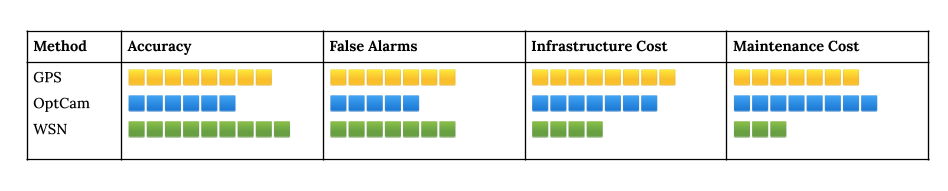
\includegraphics[width=\textwidth]{forest-fire-detection-comparison.png}
%         \caption{Comparison between different forest fire detection techniques}
%         \label{fig:forest_fire_comparison}
%     \end{figure}
% }

\only<2>{
    The WSN is built using \textsc{MaxLST} concepts-
    \begin{enumerate}
         \item{A connected network with a clustered hierarchical topology is developed}
        \item{The number of cluster nodes is controlled}
        \item{Which nodes should lie on the communication backbone}
    \end{enumerate}
}

% \only<4>{
%     \begin{figure}
%         \centering
%         \includegraphics[height=0.4\linewidth]{forest-graph-1.png}
%         \caption{Graph representation of a forest network}
%     \end{figure}
% }

\only<3>{
    \begin{figure}
        \centering
        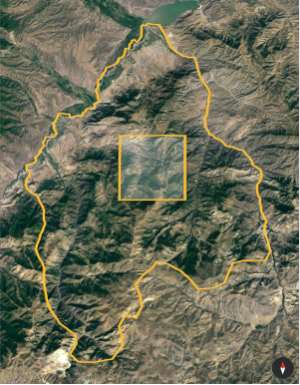
\includegraphics[height=0.6\textwidth]{forest_fire_1.png}
        \caption{Arasbaran forest and the highlighted simulation area}
    \end{figure}
}

\only<4>{
    \begin{figure}
        \centering
        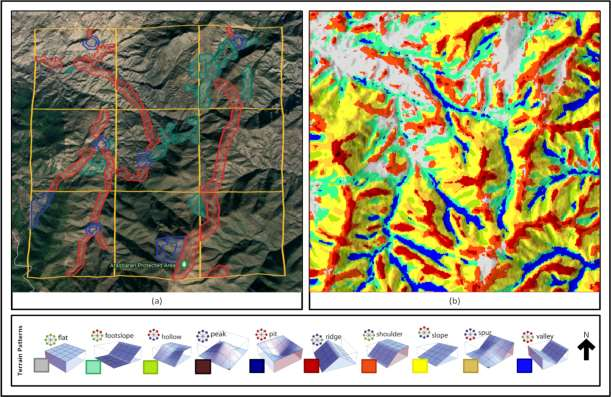
\includegraphics[width=0.8\textwidth]{forest_fire_2.png}
        \caption{3D satellite image of the simulation area with high risk of fire ignition}
    \end{figure}
}

\only<5>{
    \begin{figure}
        \centering
        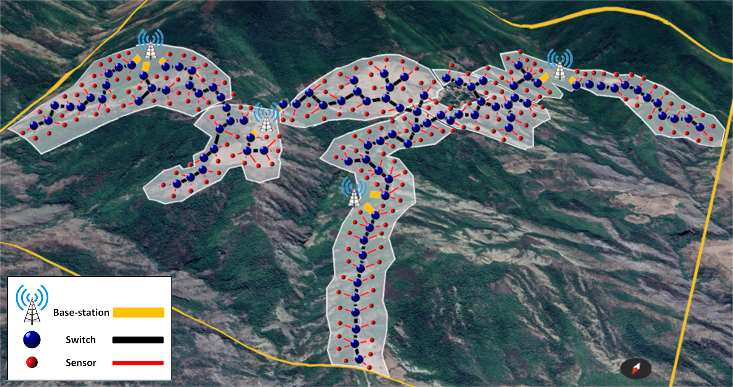
\includegraphics[width=\textwidth]{forest_fire_3.png}
        \caption{Optimum output of the sensor network of the simulation area}
    \end{figure}
}

\end{frame}

\section{Exact Algorithm}

%% setting footnote size to tiny
\setbeamerfont{footnote}{size=\tiny}

\begin{frame}{Exact Algorithm}
    \begin{itemize}
        \item An exact algorithm with running time $O({1.8966}^{n})$
        \item Proposed by Fernau et al. 2011 \footnote{Henning Fernau, Joachim Kneis, Dieter Kratsch, Alexander Langer, Mathieu Liedloff, Daniel Raible, Peter Rossmanith, \textit{An exact algorithm for the Maximum Leaf Spanning Tree problem}, Theoretical Computer Science, Volume 412, Issue 45, 2011, Pages 6290-6302, ISSN 0304-3975, \href{https://doi.org/10.1016/j.tcs.2011.07.011}{\url{https://doi.org/10.1016/j.tcs.2011.07.011}}}
    \end{itemize}
\end{frame}

%% setting footnote size back to normal
\setbeamerfont{footnote}{size=\footnotesize}

\begin{frame}{Exact Algorithm}
    \only<1>{
        \begin{figure}
            \centering
            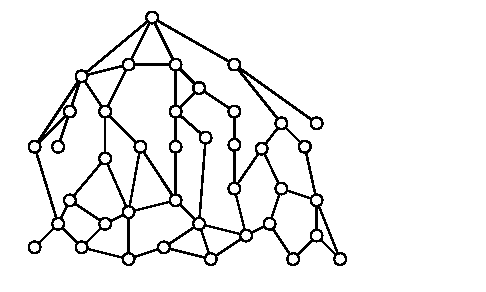
\includegraphics[width=0.9\linewidth]{original-graph-fernau.pdf}
            \caption{An example of a graph $G$}
            \label{fig:orig-graph-fernau}
        \end{figure}
    }
    \only<2>{
        \begin{figure}
            \centering
            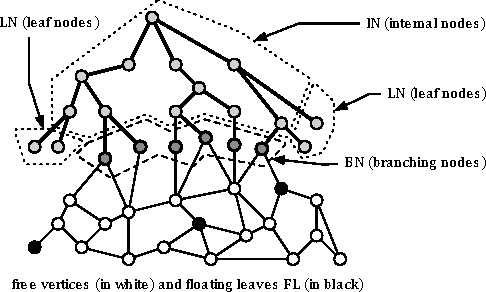
\includegraphics[width=0.9\linewidth]{subtree-graph-fernau.pdf}
            \caption{$G$ with a subtree with corresponding sets of vertices IN, BN, LN (describing the subtree), as well as FL and Free.}
            \label{fig:subtree-graph-fernau}
        \end{figure}
    }
\end{frame}

\begin{frame}{Degree of a node}
    do we need a slide for this or just explain from the previous figure?
\end{frame}

\begin{frame}{Reduction Rules: R1}
    \only<1>{
        \begin{figure}
            \centering
            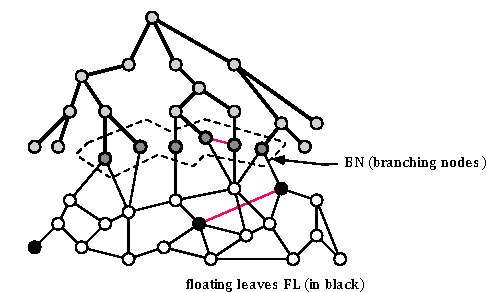
\includegraphics[width=0.6\linewidth]{R1-1.pdf}
            \caption{Reduction Rules: R1}
            \label{fig:R1-1}
        \end{figure}
    }
    \only<2>{
        \begin{figure}
            \centering
            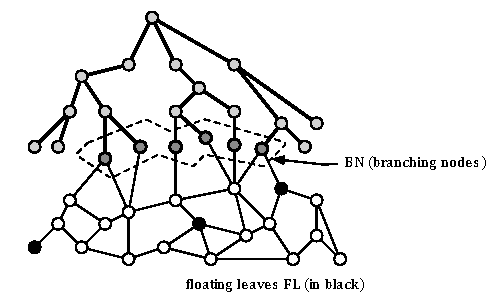
\includegraphics[width=0.6\linewidth]{R1-2.pdf}
            \caption{Reduction Rules: R1}
            \label{fig:R1-2}
        \end{figure}
    }
    \only<1-2>{
        \begin{block}{R1}
            If there exist two adjacent vertices $u, v \in V$ such that $u, v \in \text{FL}$ or $u, v \in \text{BN}$, then remove the edge $\{u, v\}$ from $G$.
        \end{block}
    }
\end{frame}

\begin{frame}{Reduction Rules: R2}
    \only<1>{
        \begin{figure}
            \centering
            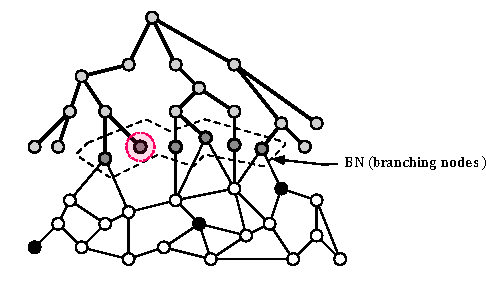
\includegraphics[width=0.6\linewidth]{R2.pdf}
            \caption{Reduction Rules: R2}
            \label{fig:R2}
        \end{figure}
    }
    \only<1>{
        \begin{block}{R2}
            If there exists a node $v \in \text{BN}$ with $d(v) = 0$, then move $v$ into $\text{LN}$.
        \end{block}
    }
\end{frame}

\begin{frame}{Reduction Rules: R3}
    \only<1>{
        \begin{figure}
            \centering
            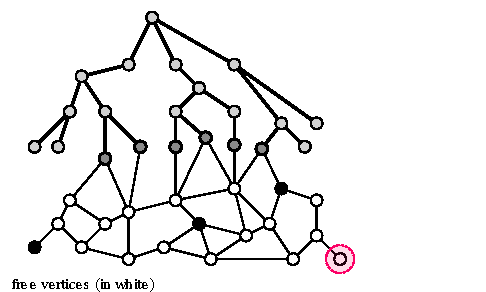
\includegraphics[width=0.6\linewidth]{R3.pdf}
            \caption{Reduction Rules: R3}
            \label{fig:R3}
        \end{figure}
    }
    \only<1>{
        \begin{block}{R3}
            If there exists a free vertex $v$ with $d(v) = 1$, then move $v$ into FL.
        \end{block}
    }
\end{frame}

\begin{frame}{Reduction Rules: R4}
    \only<1>{
        \begin{figure}
            \centering
            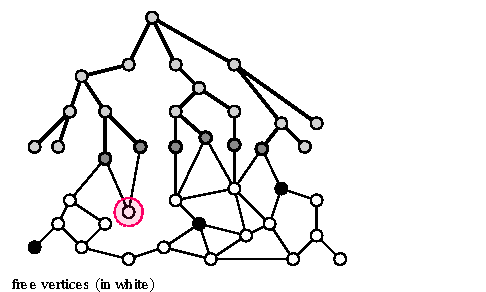
\includegraphics[width=0.6\linewidth]{R4.pdf}
            \caption{Reduction Rules: R4}
            \label{fig:R4}
        \end{figure}
    }
    \only<1>{
        \begin{block}{R4}
            If there exists a free vertex $v$ with no neighbors in $\text{Free} \cup \text{FL}$, then move $v$ into FL.
        \end{block}
    }
\end{frame}

\begin{frame}{Reduction Rules: R5}
    \only<1>{
        \begin{figure}
            \centering
            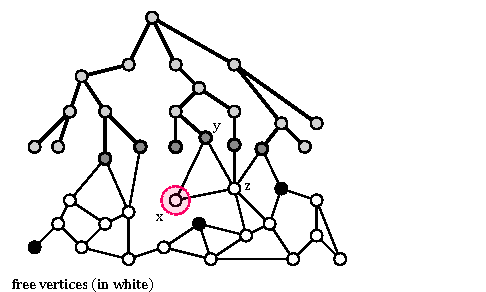
\includegraphics[width=0.6\linewidth]{R5.pdf}
            \caption{Reduction Rules: R5}
            \label{fig:R5}
        \end{figure}
    }
    \only<1>{
        \begin{block}{R5}
            If there exists a triangle $\{x, y, z\}$ in $G$ with $x$ a free vertex and $d(x) = 2$, then move $x$ into FL.
        \end{block}
    }
\end{frame}

\begin{frame}{Reduction Rules: R6}
    \only<1>{
        \begin{figure}
            \centering
            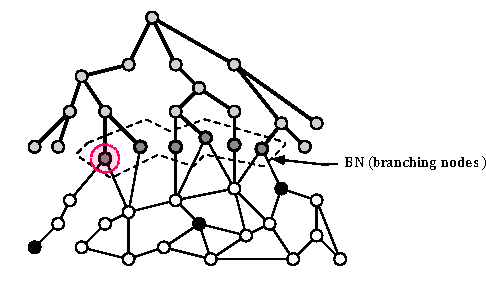
\includegraphics[width=0.6\linewidth]{R6.pdf}
            \caption{Reduction Rules: R6}
            \label{fig:R6}
        \end{figure}
    }
    \only<1>{
        \begin{block}{R6}
             If there exists a node $u \in \text{BN}$ which is a cut vertex in $G$, then apply rule $u \rightarrow \text{IN}$.
        \end{block}
    }
\end{frame}

\begin{frame}{Reduction Rules: R7}
    \only<1>{
        \begin{figure}
            \centering
            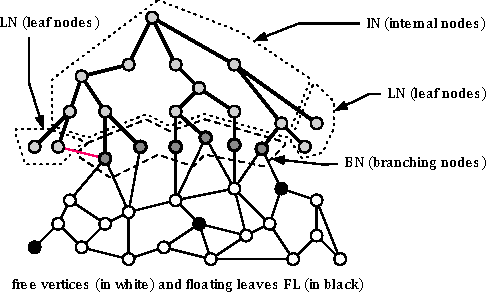
\includegraphics[width=0.6\linewidth]{R7-1.pdf}
            \caption{Reduction Rules: R7}
            \label{fig:R7-1}
        \end{figure}
    }
    \only<2>{
        \begin{figure}
            \centering
            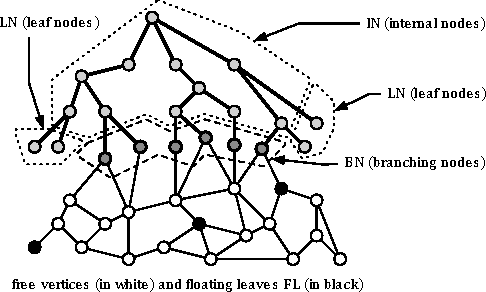
\includegraphics[width=0.6\linewidth]{R7-2.pdf}
            \caption{Reduction Rules: R7}
            \label{fig:R7-2}
        \end{figure}
    }
    \only<1-2>{
        \begin{block}{R7}
              If there exist two adjacent vertices $u, v \in V$ such that $u \in \text{LN}$ and $v \in V \setminus \text{IN}$, then remove the edge $\{u, v\}$ from $G$.
        \end{block}
    }
\end{frame}

\section{2-Approximation Algorithm}


\begin{frame}{2-Approximation Algorithm}
 % $G$ is a simple, undirected graph. We start with an empty subgraph $F$, and incrementally expand $F$ until it forms a spanning tree of $G$ with an approximation ratio of 2.
\bigskip
\begin{itemize}[<+->]
    \item $G$ is a simple, undirected graph.
    \item We start with an empty subgraph $F$, and incrementally expand $F$ until it forms a spanning tree of $G$.
    \item $F$ has all the vertices of $G$.
    \item The set of edges of $F$ is a subset of the set of edges of $G$.
\end{itemize}
\end{frame}


\begin{frame}{Expanding a Vertex in a Graph}
% Let $G$ be a graph and let $F$ be a (possibly empty) subgraph of $G$.
\bigskip

The operation of expanding a vertex $v \in V(G)$ consists of the following steps:

\begin{enumerate}
    \item If $v \notin V(F)$, add $v$ to $F$.
    \item For every $w \in N_G(v) \setminus V(F)$, add vertex $w$ and edge $vw$ to $F$.
\end{enumerate}

\bigskip

Note that:
\begin{itemize}
    \item $N_G(v)$ denotes the neighborhood of $v$ in $G$, i.e., the set of vertices adjacent to $v$.
    \item $V(G) \setminus S$ denotes the set of vertices in $G$ that are not in $S$.
\end{itemize}
\end{frame}



\begin{frame}{Expansion Rules}
\begin{itemize}
    \item We use four expansion rules, where the given order defines the priorities. 
    \item for any $i < j$, if Rule $i$ can be applied, then Rule $j$ may not be applied.
\end{itemize}

\end{frame}

\begin{frame}{Expansion Rules}
\begin{exampleblock}{Rule 1}
 If $F$ contains a vertex $v$ with at least two neighbors in $\overline{V(F)}$, then expand $v$.
\end{exampleblock}
\begin{figure}
    \centering
    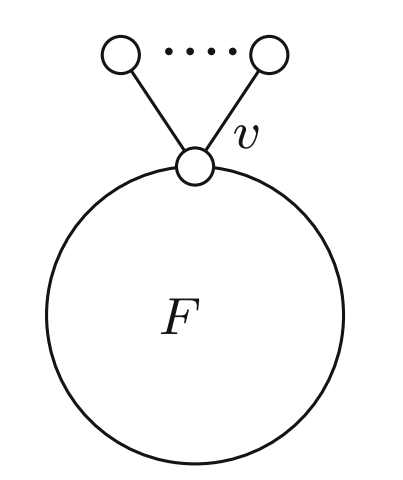
\includegraphics[height=0.3\textwidth]{rule1.png}
    \caption{Rule 1}
\end{figure}
\end{frame}


\begin{frame}{Expansion Rules}
\begin{exampleblock}{Rule 2}
 If $F$ contains a vertex $v$ with only one neighbor $w$ in $\overline{V(F)}$, which in turn has at least three neighbors in $\overline{V(F)}$, then first expand $v$, and next expand $w$.
\end{exampleblock}
\begin{figure}
    \centering
    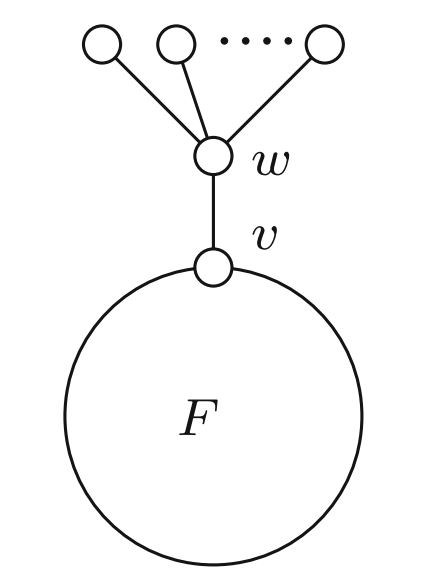
\includegraphics[height=0.3\textwidth]{rule2.png}
    \caption{Rule 2}
\end{figure}
\end{frame}


\begin{frame}{Expansion Rules}

\bigskip

\begin{exampleblock}{Rule 3}
 If $F$ contains a vertex $v$ with only one neighbor $w$ in $\overline{V(F)}$, which in turn has two neighbors in $\overline{V(F)}$, then first expand $v$, and next expand $w$.
\end{exampleblock}
\begin{figure}
    \centering
    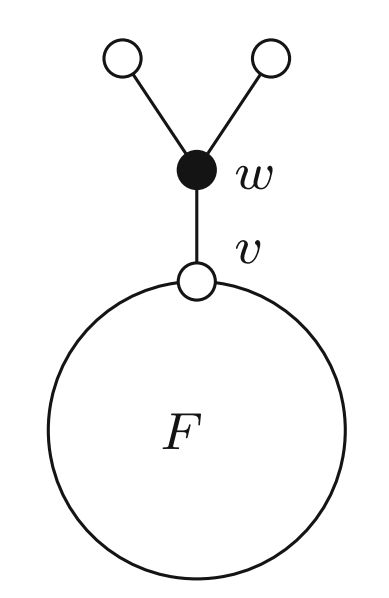
\includegraphics[height=0.3\textwidth]{rule3.png}
    \caption{Rule 3}
\end{figure}
\end{frame}

\begin{frame}{Expansion Rules}
\begin{exampleblock}{Rule 4}
If $\overline{V(F)}$ contains a vertex $v$ with at least three neighbors in $\overline{V(F)}$, then expand $v$.
\end{exampleblock}
\begin{figure}
    \centering
    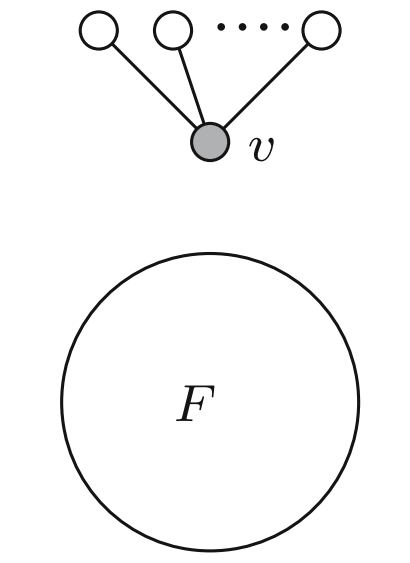
\includegraphics[height=0.3\textwidth]{rule4.png}
    \caption{Rule 4}
\end{figure}
\end{frame}


\begin{frame}{Expansion Rules}
\begin{columns}
    \begin{column}{0.7\textwidth}
        \begin{itemize}[<+->]
            \item Only Rule 4 increases the number of components of F.
            \item The priorities ensure that when Rule 4 is applied,
Rules 1, 2, and 3 cannot be applied to any component of F.
            \item Once a new component is introduced, existing components
of F will not be modified anymore.
        \end{itemize}
    \end{column}
    \begin{column}{0.3\textwidth}
        \begin{figure}
            \scalebox{1.3}{
            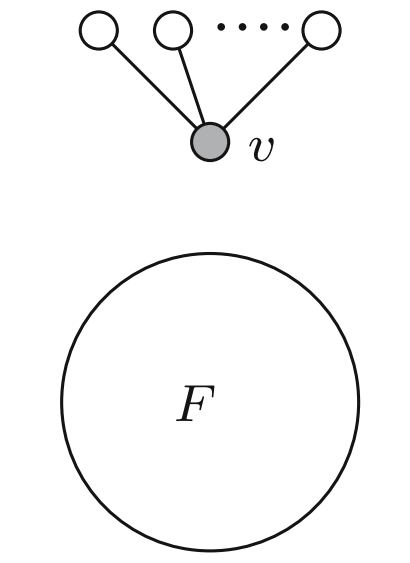
\includegraphics[height=0.5\textwidth]{rule4.png}
            }
            \caption{Rule 4}
        \end{figure}
    \end{column}
\end{columns}
\end{frame}

\begin{frame}{Finally}
\begin{itemize}
    \item Choose an edge of $G$ between different components of $F$, and add it to $F$.
\end{itemize}
\end{frame}


\begin{frame}{Algorithm}
    \begin{algorithm}[H]\footnotesize
    \SetAlgoLined
    \KwData{A connected simple undirected graph $G$ with maximum degree at least 3.}
    \KwResult{A spanning tree $T^*$ of $G$.}
    // First phase:\
    \\$F :=$ the empty graph.\
    \\\While{one of the Expansion Rules 1-4 can be applied to $F$}{
    Apply the expansion rule with the highest priority to $F$.\
    }
    $F^* := F$\
    \\// Second phase:\
    \\\While{$F$ is not spanning}{
    Choose a vertex $v \in V(F)$ with $N_G(v) \setminus V(F) \neq \emptyset$, and expand $v$.\
    }
    \While{$F$ is not connected}{
    Choose an edge of $G$ between different components of $F$, and add it to $F$.\
    }
    $T^* := F$\
    \\\Return{$T^*$}\
    % \caption{Algorithm for finding a spanning tree $T^$ of a connected simple undirected graph $G$ with maximum degree at least 3.}
    
    \end{algorithm} 
\end{frame}

\begin{frame}{Time Complexity}
    \begin{exampleblock}{Data Structure}
        \begin{itemize}
            \item G is represented using adjacency lists.
            \item Total 4 doubly link lists for 4 expansion rules candidates (R1 to R4).
            \begin{itemize}
                \item R1 contains all vertices in $v \in V(F)$ that have at least two neighbors in $\overline{V(F)}$.
                \item R2 contains all vertices $w \in$ $\overline{V(F)}$ that have at least one neighbor v in V(F), and at least three neighbors in $\overline{V(F)}$.
                \item R3 contains all vertices $w \in$ $\overline{V(F)}$ that have at least one neighbor v in V(F), and exactly two neighbors in $\overline{V(F)}$.
                \item R4 contains all vertices $w \in$ $\overline{V(F)}$ that have no neighbors in V(F), and have $d_G(w) \geq 3$.
            \end{itemize}
        \end{itemize}
        
    \end{exampleblock}
    
\end{frame}

\begin{frame}{Time Complexity}
    \begin{exampleblock}{Each vertex has}
        \begin{itemize}
            \item list number (it appears in at most one of these lists).
            \item a pointer to the corresponding doubly linked list to its position.
            \item out-degree (number of neighbors outside F).
            \item a flag for whether it is in F or not.
        \end{itemize}
    \end{exampleblock}
\end{frame}


\begin{frame}{Time Complexity}
    \begin{exampleblock}{lemma 12}
        Consider one iteration of the while-loop in the first phase of Algorithm 1.
Selecting the next vertex $w$ to expand, applying the corresponding expansion rule, and updating all data structures, can be done in time $O(d_{G}(w) + \sum_{y \in N_G(w) \setminus V(F)} d_{G}(y))$.
    \end{exampleblock}
\end{frame}

\begin{frame}{Time Complexity}
    \textbf{Phase 1:}
    \begin{columns}
    \begin{column}{0.6\textwidth}
    \begin{itemize}[<+->]
            \item First select minimum $i$ such that $R_i$ is not empty.
            \begin{itemize}
                \item constant time
            \end{itemize}
            \item Expand $w$: $O(d_G(w))$ time 
            \begin{itemize}
                \item this operation also adds all the neighbors of w.
            \end{itemize}
            \item Update out degree: For every vertex $y$ added in $F$, and for every $x$ in $N(y) \setminus F$, we update the out-degree of $x$ by subtracting 1: $\text{outdegree}[x] \gets \text{outdegree}[x] - 1$.
            \item total time (update out-degree): $O(d(w)) + \sum\limits_{y \in N(w) \setminus F} d(y)$
        \end{itemize}
        \end{column}
        \begin{column}{0.4\textwidth}
        \begin{figure}
            \scalebox{1.3}{
            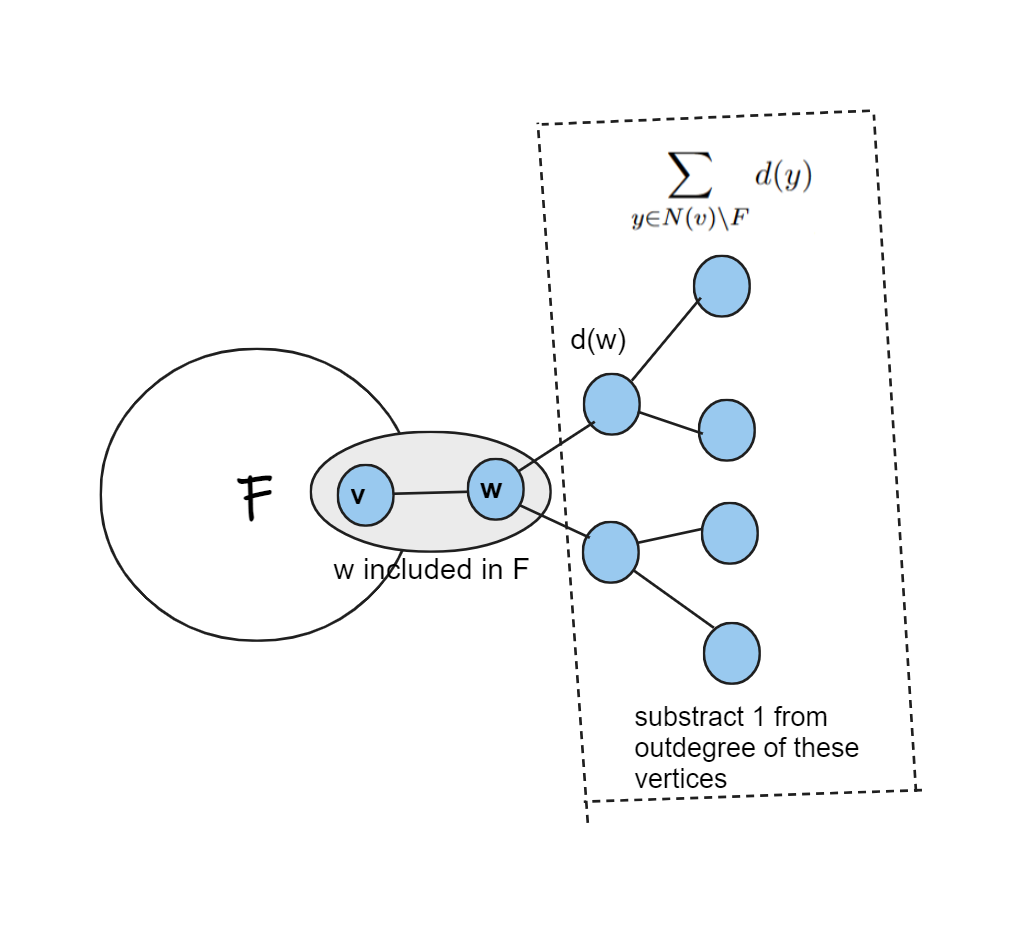
\includegraphics[height=0.8\textwidth]{outdegree.png}
            }
            
        \end{figure}
    \end{column}
\end{columns}
        
\end{frame}


\begin{frame}{Time Complexity}
    \begin{itemize}[<+->]
        \item For every vertex x, it can be verified that we can move it from one list to another in constant time.
        \item Any vertex x that has been added to F has to be removed from $R_2$, $R_3$, $R_4$ to $R_1$ if $outdegree[x] >= 2$.
        \item Any vertex x that has not been added to F but $outdegree[x]$ has been modified is first removed from the previous list and then added to $R_2$ if $outdegree[x]>=3$ or added to $R_3$ if $outdegree[x]=2$.
        \item So we never need to add vertices to $R_4$.
        \item Since adding and removing from the lists can be done in constant time.
        \item Updating the list can be done in $O(d(w)) + \sum\limits_{y \in N(w) \setminus F} d(y)$ time.
    \end{itemize}    
\end{frame}

\begin{frame}{Time Complexity}
    % G has a maximum degree at most 2, then an optimal tree can trivially be found in linear time. Otherwise, we use Algorithm 1.\\
    
    Since every vertex of $G$ can be added to $F$ at most once and expanded at most once, the total time is given by:

    \begin{align*}
    & \sum\limits_{v \in V(G)} \left(O(d(v)) + \sum\limits_{y \in N(v) \setminus F} d(y)\right) \
    \leq & \sum\limits_{v \in V(G)} 2d(v) \
    \leq & 4m \qquad \qquad \qquad \qquad \qquad (\text{where } m \text{ is the number of edges})
    \end{align*}
    
\end{frame}

\begin{frame}{Time Complexity}
    \textbf{Second Phase:}
    Analog linear Time.\\
    \textbf{Third Phase:}\\
    Let $k$ be the number of connected components of $F$, and let $g(v) \in {1,\dots,k}$ denote the connected component of $F$ that contains vertex $v$. Then, for all edges $uv$ in $G$ such that $g(u) \neq g(v)$, we can identify them and translate the problem to finding a minimum spanning tree of an auxiliary multigraph $G'$ with vertex set $|V'| \leq |V|=n$ and edge set $|E'| \leq |E|=m$. This can be solved in $O(m+n)$ time using breadth-first search.
    
\end{frame}

\begin{frame}{}
    \centering
    {\Huge Thank You}
\end{frame}


\end{document}
